\subsection{Pengujian Komponen \textit{Resource Controller}}

Pada bagian ini akan dijelaskan tentang tujuan, skenario, hasil, dan analisis dari pengujian komponen \textbf{\textit{Resource Controller}}.

\subsubsection{Tujuan Pengujian}

Tujuan pengujian ini memastikan komponen \textbf{\textit{Resource Controller}} dapat berjalan dengan baik dan menghasilkan data yang sesuai dengan ekspektasi.

\subsubsection{Skenario Pengujian}

\textbf{\textit{Resource Controller}} adalah komponen \textit{low-level} yang hanya akan digunakan oleh komponen lain. Sehingga, untuk melakukan pengujian ini, akan dilakukan dengan pendekatan pembuatan \textit{test driver} khusus. Pengujian terhadap komponen \textbf{\textit{Resource Controller}} dilakukan dengan beberapa skenario sebagai berikut.
\begin{enumerate}
    \item Mengubah alokasi prosesor maupun memori.
    \item Memastikan sistem antrian pengubahan alokasi berjalan dengan benar.
\end{enumerate}

\subsubsection{Hasil Pengujian dan Analisis}

% \begin{figure}[h]
%     \centering
%     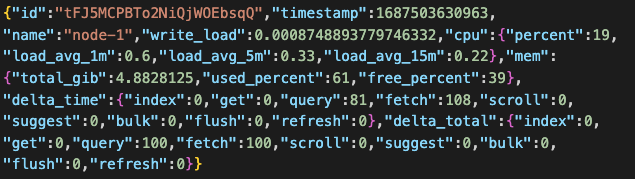
\includegraphics[width=0.8\textwidth]{chapter-4/mf-3.png}
%     \caption{Hasil Pengujian Komponen \textit{Metrics Fetcher} Skenario 3}
%     \label{fig:mf-3}
% \end{figure}

Pengujian komponen \textbf{\textit{Resource Controller}} sudah sesuai ekspektasi dan dapat dilanjutkan ke pengujian komponen lainnya.